% Created 2023-01-12 Πεμ 18:53
% Intended LaTeX compiler: pdflatex
\documentclass[11pt]{article}
\usepackage[utf8]{inputenc}
\usepackage[T1]{fontenc}
\usepackage{graphicx}
\usepackage{longtable}
\usepackage{wrapfig}
\usepackage{rotating}
\usepackage[normalem]{ulem}
\usepackage{amsmath}
\usepackage{amssymb}
\usepackage{capt-of}
\usepackage{hyperref}
\usepackage{booktabs}
\usepackage{import}
\usepackage[LGR, T1]{fontenc}
\usepackage[greek, english]{babel}
\usepackage{alphabeta}
\usepackage{esint}
\usepackage{mathtools}
\usepackage{esdiff}
\usepackage{makeidx}
\usepackage{glossaries}
\usepackage{newfloat}
\usepackage{minted}
\usepackage{chemfig}
\usepackage{svg}
\usepackage[a4paper, margin=3cm]{geometry}
\author{Βιδιάνος Γιαννίτσης}
\date{\today}
\title{Ανάλυση του block 300 - Λέβητας Λιγνίνης}
\hypersetup{
 pdfauthor={Βιδιάνος Γιαννίτσης},
 pdftitle={Ανάλυση του block 300 - Λέβητας Λιγνίνης},
 pdfkeywords={},
 pdfsubject={},
 pdfcreator={Emacs 28.2 (Org mode 9.5.5)}, 
 pdflang={English}}
\makeatletter
\newcommand{\citeprocitem}[2]{\hyper@linkstart{cite}{citeproc_bib_item_#1}#2\hyper@linkend}
\makeatother

\usepackage[notquote]{hanging}
\begin{document}

\maketitle
\tableofcontents

\renewcommand{\abstractname}{Περίληψη}
\renewcommand{\tablename}{Πίνακας}
\renewcommand{\figurename}{Σχήμα}
\renewcommand\listingscaption{Κώδικας}

\section{Διάγραμμα ροής και επεξήγηση}
\label{sec:orgcc79510}
\begin{figure}[htbp]
\centering
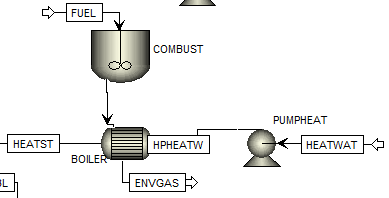
\includegraphics[width=.9\linewidth]{/home/vidianos/Documents/7o_εξάμηνο/Σχεδιασμός_Ι/Project/git_repo/Final_exam_files/Block_300_-_Λέβητας_Καύσης_Λιγνίνης/2023-01-10_18-51-18_screenshot.png}
\caption{Διάγραμμα Ροής του block 300}
\end{figure}

Στο block 300 παρουσιάζεται ο λέβητας της εγκατάστασης ο οποίος χρησιμοποιεί την λιγνίνη ως καύσιμο. Σκοπός του είναι η παραγωγή ατμού υψηλής πίεσης για χρήση ως θερμαντικό μέσο. Επίσης όμως, μπορεί να χρησιμοποιηθεί και για ηλεκτροπαραγωγή σε μία διάταξη όπως το κύκλο Rankine. Αυτό δεν υπάρχει ακόμη κάπου στην προσομοίωση, αλλά έχει θεωρηθεί πως όση από την ηλεκτρική ενέργεια μπορεί να παραχθεί από την λιγνίνη θα παραχθεί.

\section{Σχεδιαστικές Επιλογές}
\label{sec:org7a35905}
Οι βασικές σχεδιαστικές επιλογές του λέβητα, είναι η πίεση στην οποία θα λειτουργεί ο λέβητας (πίεση εισόδου του νερού στον εναλλάκτη), ο βαθμός υπερθέρμανσης του λέβητα και οι συνθήκες λειτουργίας και ο τύπος του αντιδραστήρα.

Ο αντιδραστήρας που επιλέχθηκε είναι CSTR καθώς θέλουμε αντιδραστήρα συνεχούς ροής, για να υπάρχει συνεχή ροή καυσαερίων και άρα ατμοπαραγωγή που είναι το αποτέλεσμα του block αυτού. Ο CSTR αντιδραστήρας είναι η πιό απλή περίπτωση αντιδραστήρα συνεχούς ροής στην ανάλυση του και καθώς δεν είναι και από τους βασικούς αντιδραστήρες της διεργασίας, δεν έχουμε ασχοληθεί με πιθανά θέματα βελτιστοποίησης του. Ο αντιδραστήρας λειτουργεί σε πίεση 1 bar μη ισοθερμοκρασιακά. Η θερμογόνος δύναμη της λιγνίνης είναι γνωστή από βιβλιογραφία \textsuperscript{\citeprocitem{1}{1}} άρα μπορεί από αυτήν να υπολογιστεί η θερμοκρασία λειτουργίας του αντιδραστήρα η οποία είναι 1822 \(^oC\). Ο υπολογισμός έγινε στο χέρι και αποτελεί την αδιαβατική θερμοκρασία φλόγας και όχι την πραγματική. Όμως, ότι προσπάθεια έγινε να γίνει η προσομοίωση με δεδομένο heat duty και όχι θερμοκρασία έδινε errors, για αυτό ακολουθήθηκε αυτή η προσέγγιση. Επίσης πολύ σημαντικό σχεδιαστικό δεδομένο για έναν καυστήρα, είναι η περίσσεια άερα. Βρέθηκε σε βιβλιογραφία πως για την καύση πυρηνόξυλου, χρησιμοποιείται μία περίσσεια αέρα λ = 2.5. Παρόλο που η καύση γίνεται μόνο με την λιγνίνη και όχι όλο το πυρηνόξυλο, η τιμή του λ αυτή αναμένεται να είναι αρκετά κοντά άρα θεωρήθηκε μία περίσσεια αέρα της τάξης αυτής.

Ο λέβητας τώρα έχει ως σκοπό την παραγωγή ατμού υψηλής πίεσης, αφού τα καυσαέρια έχουν πολύ υψηλό θερμικό περιεχόμενο και μπορούν να παράξουν αυτόν τον ατμό. Η τιμή της πίεσης επιλέχθηκε στα 4 MPa η οποία είναι μία κλασσική πίεση λειτουργίας σε λέβητες υψηλής πίεσης. Η θερμοκρασία κορεσμού του ατμού στην πίεση αυτή είναι 250.4 \(^oC\). Ένας λέβητας παράγει τυπικά ελαφρώς υπέρθερμο ατμό, καθώς σε αρκετές περιπτώσεις (όπως στην ηλεκτροπαραγωγή), αυτός οδηγείται σε στρόβιλο στον οποίο πρέπει να μπαίνει υπέρθερμος ατμός και αν παραχθεί καθόλου μίγμα υγρού-ατμού αυτό να έχει υψηλή ποιότητα. Σε άλλη περίπτωση, θα υπάρξει μηχανολογικό πρόβλημα. Μέχρι τώρα, δεν υπάρχει κάτι τέτοιο στην διεργασία μας για να έχουμε μία καλή προσέγγιση του βαθμού υπερθέρμανσης που θέλουμε, για αυτό θεωρήθηκε ένας βαθμός υπερθέρμανσης του ατμού, λίγο πάνω από την θερμοκρασία κορεσμού του. Επιλέχθηκε αυθαίρετα η θερμοκρασία εξόδου 259 \(^oC\). 

\section{Υπολογισμοί}
\label{sec:orgf81babd}
Οι βασικοί υπολογισμοί της διεργασίας είναι η δυναμικότητα του λέβητα (πόσο ατμό υψηλής πίεσης παράγει ανά μονάδα χρόνου) και η κινητική του αντιδραστήρα.

Για την κινητική του αντιδραστήρα, θεωρήθηκε η εξής αντίδραση καύσης για την λιγνίνη
\[  C_{7.3}H_{13.9}O_{1.3} + 10.125O_2 \rightarrow 6.95 H_2O + 7.3CO_2  \] \textsuperscript{\citeprocitem{2}{2}} και βρέθηκε πως ακολουθεί κινητική πρώτης τάξης με ενέργεια ενεργοποίησης 46.68 kJ/mol και προεκθετικό παράγοντα 12.96 h\textsuperscript{-1} ή 3.6e-3 s\textsuperscript{-1} σε μονάδες SI \textsuperscript{\citeprocitem{3}{3}} . Βέβαια, αξίζει να αναφερθεί πως η μελέτη αυτή έγινε για lignin char και όχι για καθαρή λιγνίνη.

Για την δυναμικότητα του λέβητα, ξέρουμε ότι η τροφοδοσία έχει 5169 kg/hr λιγνίνη. Αν υποθέσουμε ότι όλη η λιγνίνη καίγεται σε έναν καυστήρα και τα καυσαέρια αυτού θερμαίνουν ατμό στα 4 MPa και 259 \(^oC\) σε έναν εναλλάκτη, προκύπτει πως μπορούμε να έχουμε ένα ρεύμα εξόδου 107.2 tn/h ατμό. Αξίζει να σημειωθεί πως δεν σταματάμε την εναλλαγή όταν το ΔΤ\textsubscript{min} των ρευμάτων γίνει πολύ μικρό, αλλά όταν η θερμοκρασία των καυσαερίων φτάσει κάτω από 150 \(^oC\). Γενικά σε χαμηλές θερμοκρασίες υπάρχει η ανησυχία συμπήκνωσης ισχυρών οξέων όπως το θειικό και το νιτρικό από τα οξείδια τους που μπορεί να υπάρχουν στον καυστήρα (παρότι στην περίπτωση μας έχουν αγνοηθεί). Επίσης, σε χαμηλές θερμοκρασίες, είναι δύσκολος ο ελκυσμός του λέβητα καθώς CO\textsubscript{2} το οποίο είναι βαρύτερο από τον αέρα μπορεί να τον φρακάρει. Στην προκειμένη έχει οριστεί θερμοκρασία εξόδου καυσαερίων 110 \(^oC\), αλλά εν γένει οι περισσότερες θερμοκρασίες πάνω από 100 \(^oC\) είναι καλές, καθώς το πυρηνόξυλο είναι υλικό μηδενικού θείου \textsuperscript{\citeprocitem{4}{4}}, άρα το θειικό οξύ το οποίο είναι ο βασικός μας φόβος που πηγαίνει την θερμοκρασία αυτή στους 150 \(^oC\) δεν μπορεί να σχηματιστεί.

Στην πράξη είναι μάλλον καλύτερο να εγκαθιστάται ένας μικρότερος λέβητας σε κάθε σημείο που υπάρχει η ανάγκη για να μην διακινείται ατμός υψηλής πίεσης για μεγάλες αποστάσεις. Καθώς ο βαθμός υπερθέρμανσης δεν είναι μεγάλος, σε μεγάλη απόσταση, μπορεί η πτώση πίεσης κατά μήκος του αγωγού να κάνει τον ατμό μίγμα υγρού-ατμού το οποίο θα μείωνε την αποδοτικότητα του. Αλλά, ο υπολογισμός αυτός είναι χρήσιμος για να ξέρουμε την μέγιστη δυνατή δυναμικότητα του εργοστασίου.

Το ιδανικό θα ήταν να μπορούσαμε να ξέρουμε πόση λιγνίνη απαιτείται για την παραγωγή μίας συγκεκριμένης ποσότητας ατμού, αλλά στην παρούσα φάση αυτό δεν έχει γίνει με μία μονοσήμαντη σχέση. Θεωρούμε πως ίσως να μπορεί να γίνει στο Aspen μέσω του Calculator, αλλά δεν έχει υπάρξει χρόνος για σχετικούς πειραματισμούς.

\section{Προσομοιώσεις στο Aspen}
\label{sec:orgc3d1b0c}
Το μοντέλο που χρησιμοποιήθηκε για την προσομοίωση είναι το SRK. Η καταστατική εξίσωση SRK είναι ιδανική για τον προσδιορισμό της μη ιδανικότητας της αέριας φάσης η οποία υπάρχει και είναι σε πολλά σημεία και σε υψηλή πίεση.

Στο Aspen τα δύο ρεύματα εισόδου είναι το νερό (του οποίου ποσότητα μεταβάλλουμε για να εκμεταλλευτούμε όσο το δυνατόν περισσότερη ενέργεια των καυσαερίων) και το καύσιμο μίγμα λιγνίνης και αέρα ο οποίος είναι σε περίσσεια 2.5 φορές από τον στοιχειομετρικό. Ο αντιδραστήρας της καύσης ορίστηκε σε πίεση 1 bar και θερμοκρασία 2095.6 Κ στον οποίο γίνεται αντίδραση καθαρά στην αέρια φάση εφόσον δεν υπάρχουν υγρά. Ο όγκος του αντιδραστήρα ορίστηκε ως 60 Mm\textsuperscript{3} το οποίο βρέθηκε πως είναι όγκος που πετυχαίνει πολύ υψηλή μετατροπή της λιγνίνης. Όπως αναφέρθηκε, δεν θα χρησιμοποιηθεί στην πράξη αυτός ο αντιδραστήρας αλλά θα σπάσει σε κομμάτια άρα αυτό δεν είναι και τόσο σημαντικό. Η κινητική του ορίστηκε ως ένα power law expression με την παραπάνω στοιχειομετρία, ειδική ταχύτητα και ενέργεια ενεργοποίησης.

Το νερό οδηγείται αρχικά σε αντλία με discharge pressure 4 MPa και έπειτα οδηγείται στον εναλλάκτη όπου εναλάσσει θερμότητα με τα καυσαέρια. Από το διάγραμμα T-q που δίνει το Aspen, μπορούμε να δούμε πόσο νερό μπορούμε να βάλουμε ώστε να εκμεταλλευτούμε όλη την θερμική ενέργεια των καυσαερίων μέχρι τους 100 \(^oC\) και λίγο παραπάνω σε κάθε περίπτωση.

\section{Βιβλιογραφία}
\label{sec:org771a268}
\hypertarget{citeproc_bib_item_1}{(1) Fernandez-Bolanos, J.; Felizon, B.; Heredia, A.; Guillen, R.; Jimenez, A. Characterization of the Lignin Obtained by Alkaline Delignification and of the Cellulose Residue from Steam-Exploded Olive Stones. \textit{Bioresource technology} \textbf{1999}, \textit{68} (2), 121–132. \url{https://doi.org/10.1016/S0960-8524(98)00134-5}.}

\hypertarget{citeproc_bib_item_2}{(2) Wooley, R. J.; Putsche, V. Development of an ASPEN PLUS Physical Property Database for Biofuels Components. \textbf{1996}, 36.}

\hypertarget{citeproc_bib_item_3}{(3) Farrokh, N. T.; Suopajärvi, H.; Sulasalmi, P.; Fabritius, T. A Thermogravimetric Analysis of Lignin Char Combustion. \textit{Energy procedia} \textbf{2019}, \textit{158}, 1241–1248. \url{https://doi.org/10.1016/j.egypro.2019.01.413}.}

\hypertarget{citeproc_bib_item_4}{(4) Gonzalez, J. F.; Gonzalez-Garcia, C. M.; Ramiro, A.; Gonzalez, J.; Sabio, E.; Ganan, J.; Rodrıguez, M. A. Combustion Optimisation of Biomass Residue Pellets for Domestic Heating with a Mural Boiler. \textit{Biomass and bioenergy} \textbf{2004}, \textit{27} (2), 145–154. \url{https://doi.org/10.1016/j.biombioe.2004.01.004}.}
\end{document}